\documentclass[10pt,a4paper]{article}
\usepackage{fullpage}
\usepackage[utf8]{inputenc}
\usepackage[LGR,T1]{fontenc}
\usepackage{amsmath}
\usepackage{amssymb}
\usepackage{graphicx}
\usepackage[greek,english]{babel}
\usepackage{url}
\usepackage{hyperref}
\usepackage{listings}
\usepackage{textcomp}
\usepackage{accsupp}
\usepackage{attachfile}
\usepackage{verbatim}
\usepackage[misc]{ifsym}
\usepackage{placeins}

%\newcommand{\textgreek}[1]{\begingroup\fontencoding{LGR}\selectfont#1\endgroup}


% color def
\usepackage{color}
\definecolor{darkred}{rgb}{0.6,0.0,0.0}
\definecolor{darkgreen}{rgb}{0,0.50,0}
\definecolor{lightblue}{rgb}{0.0,0.42,0.91}
\definecolor{orange}{rgb}{0.99,0.48,0.13}
\definecolor{grass}{rgb}{0.18,0.80,0.18}
\definecolor{pink}{rgb}{0.97,0.15,0.45}

% listings
\usepackage{listings}

% General Setting of listings
\lstset{
	language=Python,
	tabsize=4,
	aboveskip=1em,
	breaklines=true,
	abovecaptionskip=-6pt,
	captionpos=b,
	escapeinside={\%*}{*)},
	frame=single,
	numbers=left,
	numbersep=8pt,
	numberstyle=\tiny,
	morekeywords=[1]{,as,assert,nonlocal,with,yield,self,True,False,None,} % Python builtin
	morekeywords=[2]{,__init__,__add__,__mul__,__div__,__sub__,__call__,__getitem__,__setitem__,__eq__,__ne__,__nonzero__,__rmul__,__radd__,__repr__,__str__,__get__,__truediv__,__pow__,__name__,__future__,__all__,}, % magic methods
	morekeywords=[3]{,object,type,isinstance,copy,deepcopy,zip,enumerate,reversed,list,set,len,dict,tuple,range,xrange,append,execfile,real,imag,reduce,str,repr,}, % common functions
	morekeywords=[4]{,Exception,NameError,IndexError,SyntaxError,TypeError,ValueError,OverflowError,ZeroDivisionError,}, % errors
	morekeywords=[5]{,ode,fsolve,sqrt,exp,sin,cos,arctan,arctan2,arccos,pi, array,norm,solve,dot,arange,isscalar,max,sum,flatten,shape,reshape,find,any,all,abs,plot,linspace,legend,quad,polyval,polyfit,hstack,concatenate,vstack,column_stack,empty,zeros,ones,rand,vander,grid,pcolor,eig,eigs,eigvals,svd,qr,tan,det,logspace,roll,min,mean,cumsum,cumprod,diff,vectorize,lstsq,cla,eye,xlabel,ylabel,squeeze,}, % numpy / math
	deletekeywords=[2]{next,set},
	deletekeywords=[3]{next,set},
	basicstyle=\ttfamily,
	backgroundcolor=\color{white},
	commentstyle=\color{darkgreen}\slshape,
	keywordstyle=\color{blue}\bfseries\itshape,
	keywordstyle=[2]\color{blue}\bfseries,
	keywordstyle=[3]\color{grass},
	keywordstyle=[4]\color{red},
	keywordstyle=[5]\color{orange},
	stringstyle=\color{darkred},
	emphstyle=\color{pink}\underbar,
	morestring=[d]{"},
	showstringspaces=false,
	upquote=true,
    literate={á}{{\'a}}1
    	{é}{{\'e}}1
    	{í}{{\'{\i}}}1
    	{ó}{{\'o}}1
    	{ú}{{\'u}}1
    	{Á}{{\'A}}1
    	{É}{{\'E}}1
    	{Í}{{\'I}}1
    	{Ó}{{\'O}}1
    	{Ú}{{\'U}}1
    	{ü}{{\"u}}1
    	{Ü}{{\"U}}1
    	{ñ}{{\~n}}1
    	{Ñ}{{\~N}}1
    	{¿}{{?`}}1
    	{¡}{{!`}}1
}

\usepackage{tikz}
\usetikzlibrary{shapes.geometric, arrows}
\tikzstyle{startstop} = [rectangle, rounded corners, minimum width=3cm, minimum height=1cm,text centered, draw=black, fill=red!30]
\tikzstyle{io} = [trapezium, trapezium left angle=70, trapezium right angle=110, minimum width=3cm, minimum height=1cm, text centered, draw=black, fill=blue!30]
\tikzstyle{process} = [rectangle, minimum width=3cm, minimum height=1cm, text centered, draw=black, fill=orange!30]
\tikzstyle{decision} = [diamond, minimum width=3cm, minimum height=1cm, text centered, draw=black, fill=green!30]
\tikzstyle{arrow} = [thick,->,>=stealth]


\makeatletter
\lst@RequireAspects{writefile}

% Use \attachfile command to add listing content as paperclip.
\lstnewenvironment{attachedlisting}[1][]{%
	\lst@BeginAlsoWriteFile{#1.txt}%
}
{%
	\lst@EndWriteFile
	\marginpar{\attachfile[appearance=false,icon=Paperclip,mimetype=text/tex]{#1.txt}}
}

% Use accsupp package to add listing content as copyable text.
\lstnewenvironment{copyablelisting}{%
	\lst@BeginAlsoWriteFile{\jobname.txt}%
}
{%
	\lst@EndWriteFile
	\let\verbatim@processline\add@lstline
	\global\let\lstfile\empty
	\verbatiminput{\jobname.txt}%
	\marginpar{(\BeginAccSupp{method=escape,ActualText={\lstfile}}\PaperPortrait\EndAccSupp{})}
}
\def\add@lstline
{\xdef\lstfile{\unexpanded\expandafter{\lstfile}\the\verbatim@line\string^^J}}
\makeatother


\title{{\huge Frases Palindrómicas}}
\date{}


\begin{document}
\maketitle


\section{Descripción}

Un \href{https://es.wikipedia.org/wiki/Pal%C3%ADndromo}{palíndromo}\footnote{\href{https://es.wikipedia.org/wiki/Palíndromo}{https://es.wikipedia.org/wiki/Palíndromo}} es una palabra, número, frase u otra secuencia de caracteres que se lee igual hacia adelante que hacia atrás, como madam, racecar. También hay palíndromos numéricos, incluidos los sellos de fecha/hora que usan dígitos cortos 11/11/11 11:11 y dígitos largos 02/02/2020. Los palíndromos de longitud de oración ignoran la capitalización, la puntuación y los límites de las palabras.

La palabra palíndromo fue introducida por Henry Peacham en 1638. Se deriva de las raíces griegas \textgreek{πάλιν} ``de nuevo'' y \textgreek{δρóμος} ``camino, dirección''; se usa una palabra diferente en griego, \textgreek{καρκινικός} ``carkinicos'' (lit. como un cangrejo) para referirse a la escritura reversible letra por letra.

\section{Objetivo}
Tienes que desarrollar un programa en Python que verifique si una cadena (una secuencia de caracteres) es un palíndromo o no. Para hacerlo, utilizarás la estructura de datos \texttt{Deque}.

Debes tener en cuenta los siguientes aspectos:

\begin{itemize}
\item Una letra con o sin acento es la misma para fines de verificación de palíndromos.
\item Puedes usar caracteres alfanuméricos y no alfanuméricos.
\item Puedes hacer uso de:
	\begin{itemize}
	\item La librería \texttt{colorama}; por ejemplo, para resaltar las posiciones donde la expresión viola la propiedad del palíndromo. Consulta la Sección \ref{sec:colorama} para obtener más información.
	\item La implementación de \texttt{deque} en la librería \texttt{collections}. Sin embargo, siéntete libre de usar la proporcionada en clase o incluso desarrollar tu propia implementación de \texttt{deque}.
	\end{itemize}
\item Puedes solicitar el texto a verificar ya sea por teclado o leyendo desde un archivo.
\end{itemize}


\section{El Programa}

El programa se dividirá en varias partes. Tendrás que crear una estructura de menú para permitir al usuario seleccionar lo que desea hacer.


\subsection{Verificar si una Palabra es un Palíndromo (2 puntos)}

Hay muchas formas de generar un verificador de palíndromos. Puedes hacerlo creando un algoritmo de entrada de cadenas de caracteres y verificando si son un palíndromo o no. La solución al problema comenzará utilizando un \texttt{Deque}.

Como sabes, podemos eliminar los caracteres en ambos lados simultáneamente, compararlos y continuar haciéndolo a menos que los caracteres difieran. Después de algunas comparaciones, solo tendrás un carácter en el \texttt{Deque}. Sin embargo, depende de la palabra si es impar o par. Verificará si la palabra es un palíndromo o no.

Implementa este algoritmo en una función llamada \lstinline|test_palindrome_word(word: str) -> bool|. Tomará una cadena que contiene una palabra como argumento y verificará si la palabra ya es un palíndromo o no, devolviendo \lstinline|True| si lo es, \lstinline|False| si no lo es.

\subsection{Verificar si una cadena es un palíndromo (1 Punto)}
Crea una nueva función llamada \lstinline|test_palindrome_string(text: str) -> bool| utilizando la anterior como ejemplo, para que pueda funcionar con cualquier oración. Ten en cuenta que para que una oración sea un palíndromo, se ignoran los espacios y los signos de puntuación.

\subsection{Resaltar los Resultados (4 Puntos)}

Puedes usar la librería \texttt{Colorama} (explicada en la Sección \ref{sec:colorama}) para resaltar los resultados. Puedes mostrar la oración en verde cuando sea un palíndromo. De lo contrario, puedes imprimir los primeros dos caracteres que rompen la regla del palíndromo en color rojo. Al mostrar la oración, ten en cuenta que debes mostrarla tal como la ingresó el usuario, no después de eliminar los espacios u otros elementos.


\subsection{Buscar la Expresión en un Archivo (1 Punto)}
%Abriremos un cuadro de diálogo del sistema para abrir un archivo en el sistema gracias a la biblioteca \texttt{easygui}. Como en el caso anterior, verificaremos si el contenido del archivo es un palíndromo o no.
%
%Solo la elección del archivo debe hacerse usando easigui. El resto, mostrar el resultado, etc., se puede hacer en la consola.

Pide al usuario que escriba la ruta de un archivo. El programa leerá el archivo y verificará si el contenido es un palíndromo. Ten cuidado al abrir el archivo, podría no existir.

\subsection{Diseñando la Aplicación}

El programa tendrá un menú principal con tres opciones diferentes:

\begin{enumerate}
\item Ingresar la expresión a verificar
\item Seleccionar un archivo para verificar
\item Salir
\end{enumerate}

\begin{figure}[h!]
\centering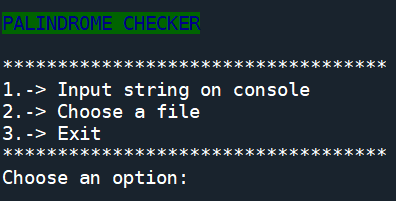
\includegraphics{img/menu}
\caption{El menú principal del programa.}
\end{figure}

\begin{figure}[h!]
\centering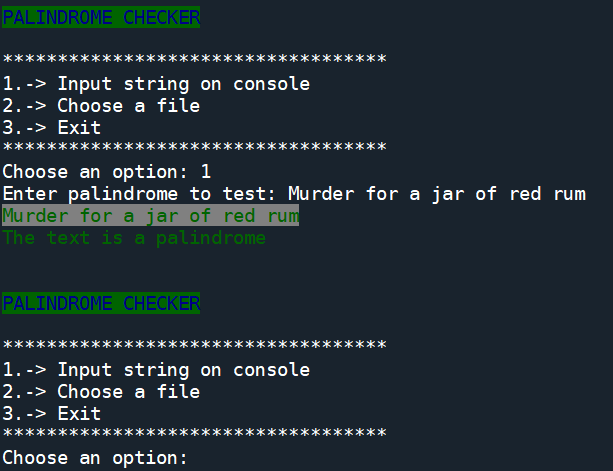
\includegraphics{img/tested}
\caption{El resultado de probar una cadena palíndroma.}
\end{figure}

\begin{figure}[h!]
\centering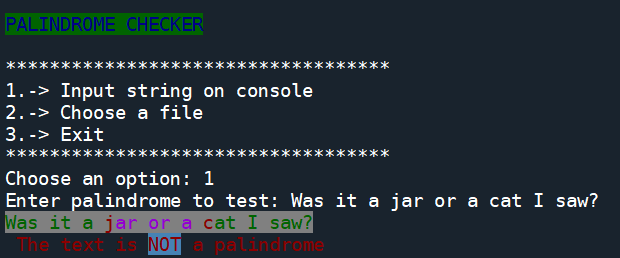
\includegraphics{img/wrong}
\caption{La cadena no es un palíndromo, el punto donde se rompe la condición se muestra en rojo.}
\end{figure}

\newpage
\null
\newpage

\subsection{Otras Observaciones}

\begin{itemize}
\item Usa funciones para estructurar tu programa y minimizar el uso de código fuera de las funciones.
    \begin{itemize}
    \item Usa la función main como el punto de entrada del programa.
\begin{attachedlisting}[main]
if __name__ == "__main__":
    main()
\end{attachedlisting}
    \end{itemize}
\end{itemize}

\subsection{Características Adicionales: (2 puntos)}
\begin{itemize}
\item Una letra con acento o sin acento es la misma para fines de verificación de palíndromos.
\item Puedes usar caracteres alfanuméricos y no alfanuméricos.
\item Cuando un usuario selecciona la opción de leer desde un archivo, en lugar de pedirle que ingrese la ruta del archivo, muestra un menú con los archivos disponibles para el usuario. Un ejemplo se puede ver en la Figura \ref{fig:file_menu}.
\item Cualquier otra adición original a tu programa.
\end{itemize}

\begin{figure}[h!]
\centering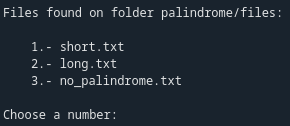
\includegraphics{img/files}
\label{fig:file_menu}
\caption{Un menú que muestra los archivos encontrados en una carpeta, el usuario puede ingresar un número para elegir el archivo.}
\end{figure}

\section{Dónde Encontrar Palíndromos}
En la página de la Wikipedia sobre los palíndromos tienes algunos ejemplos, si no puedes echar un vistazo a la página de Wiktionary sobre palíndromos: \\ \href{https://en.wiktionary.org/wiki/Appendix:English_palindromes}{https://en.wiktionary.org/wiki/Appendix:English\_palindromes}


\newpage
\section{Colorear la Salida de la Terminal en Python: el Modulo \texttt{colorama}}
\label{sec:colorama}

Una forma de crear programas más dinámicos es usar colores para enfatizar elementos en la consola. El método clásico para interactuar con la configuración de la consola es usar caracteres de escape. Ya has usado al menos uno de ellos \lstinline|'\n'|, y hay algunos que son similares:
\begin{itemize}
\itemsep0em 
\item[\texttt{\textbackslash n}:] Insertar una nueva línea
\item[\texttt{\textbackslash t}:] Insertar una tabulación
\item[\texttt{\textbackslash r}:] Retorno de carro, posiciona el cursor al principio de la línea sin agregar una nueva línea
\item[\texttt{\textbackslash b}:] Retroceso
\end{itemize}

\begin{attachedlisting}[escape]
print("normal")
print("\tUn nivel")
print("\t\tDos niveles")

print("aaaaaa", end="")
print("\rbbbbbb")
\end{attachedlisting}

Hay caracteres de escape o códigos más complejos para permitir un mayor control de la consola, por ejemplo, cambiar el color del texto:

\begin{attachedlisting}[red]
print("Texto normal")
print("\033[31m" + "Texto en rojo")
print("\033[39m") # y restablecer al color predeterminado
print("Texto normal de nuevo")
\end{attachedlisting}

Tener que recordar todos los códigos especiales es una tarea ardua, y la mayoría de ellos no son tan fáciles de ingresar en un programa. Por esta razón, tenemos la librería \href{https://pypi.org/project/colorama/}{\texttt{colorama}}\footnote{\href{https://pypi.org/project/colorama/}{https://pypi.org/project/colorama/}}. \texttt{Colorama} simplifica el uso de estos caracteres de escape proporcionando variables con nombre con sus valores ya asignados. Entonces, en lugar del código anterior, podemos hacer lo siguiente:

\begin{attachedlisting}[colorama]
from colorama import Fore
print("Texto normal")
print(Fore.RED + "Texto en rojo")
print(Fore.RESET) # y restablecer al color predeterminado
print("Texto normal de nuevo")
\end{attachedlisting}

\texttt{Colorama} proporciona principalmente 3 clases diferentes que podemos importar en nuestros archivos:

\begin{description}
\itemsep0em 
\item[Fore:] Establece el color del primer plano (texto)
\begin{itemize}
\item \texttt{BLACK, RED, GREEN, YELLOW, BLUE, MAGENTA, CYAN, WHITE, RESET}
\end{itemize}
\item[Back:] Establece el color de fondo
\begin{itemize}
\item \texttt{BLACK, RED, GREEN, YELLOW, BLUE, MAGENTA, CYAN, WHITE, RESET}
\end{itemize}
\item[Style:] Algunas modificaciones globales
\begin{itemize}
\item \texttt{DIM, NORMAL, BRIGHT, RESET\_ALL}
\end{itemize}
\end{description}

\newpage

Ten en cuenta que todos los valores que proporciona \texttt{colorama} son cadenas y se pueden combinar con otras cadenas como de costumbre. Un ejemplo más completo:
\begin{attachedlisting}[example]
from colorama import Fore, Back, Style
# Establecer el color de forma semi-permanente
print(Fore.CYAN) # Observa que se inserta un salto de línea
print("El texto seguirá siendo cian")
print("hasta que se restablezca o cambie")
print(Style.RESET_ALL)  # Observa que se inserta un salto de línea
# Colorear una sola línea y luego restablecer
print(Fore.RED + 'Puedes colorear una sola línea.' + Style.RESET_ALL)
# Colorear una sola palabra en la salida
print('O una sola ' + Back.GREEN + 'palabra' + Style.RESET_ALL + ' puede ser resaltada')
# Combinar color de primer plano y de fondo
print(Fore.BLUE + Back.WHITE)
print('El primer plano, el fondo y los estilos se pueden combinar')
print("==========")
print(Style.RESET_ALL)  # Observa que se inserta un salto de linea
print('Si no estás seguro, restablece todo a la normalidad.')
\end{attachedlisting}

\subsection{Algunas Desventajas}

No todos los códigos de escape funcionan en todos los tipos de terminal. Dependen en gran medida del sistema operativo (Windows, Linux o MacOs) y del programa de terminal que se utilice. \texttt{Colorama} promete que el estilo \texttt{Fore} y \texttt{Back} debería funcionar en cualquier lugar, pero otros, por ejemplo \texttt{Style.DIM}, no funcionarán en Windows.

Puedes leer más sobre cómo funciona la librería en su página web del proyecto: \\
\href{https://pypi.org/project/colorama/}{https://pypi.org/project/colorama/}

\subsection{Instalando \texttt{colorama}}
 
Para usar la librería primero tenemos que instalarla en nuestras computadoras. Para hacer esto, podemos usar la consola que proporciona Spyder. Usaremos la utilidad \lstinline|pip| para instalar las librerías necesarias, en sus computadoras, dependiendo de su instalación de Python, es posible que tengan que usar \lstinline|conda|, el comando debería ser el mismo, simplemente cambien una palabra por la otra.

\begin{lstlisting}
pip install colorama
\end{lstlisting}

Si la instalación es exitosa, Spyder nos dirá que es posible que necesitemos reiniciar el kernel. Esto se hace haciendo clic derecho en el nombre de la pestaña de la consola en la parte superior derecha de la consola y eligiendo la opción de reiniciar el kernel.

\end{document}